\section{问题三的模型建立与求解}

\subsection{日内新信息下的求解思路}

问题三在问题二的基础上增加了新的信息和新的代价：每天0:00先制定购电计划，
6:00、12:00和18:00还能获得新的光伏预报，并允许修改尚未执行的订单，
但修改订单本身需要付费。因此，本问的关键不只是提高预测精度，
而是判断新的信息是否值得转化为新的购电订单。

新预报并不意味着必须修改订单。若预测变化较小，电池可以自行吸收偏差，
则修改订单反而可能增加费用；若预计缺口较大、储能又不足，
提前调整订单则可能比事后按5倍电价紧急购电更加经济。

针对这一特点，本文设置四种候选方案：
\begin{enumerate}
    \item 直接采用官方光伏预报；
    \item 利用历史误差融合官方预报；
    \item 采用提升树修正官方预报；
    \item 在融合预报基础上加入近期误差准备。
\end{enumerate}

四种方案均采用相同的日内滚动调度方式，并以全年实际购电费用作为最终评价依据。
综合预报信息的可解释性和紧急购电风险，本文重点研究并最终采用
\[
\boxed{\text{历史融合预报--动态安全准备--日内滚动规划模型}}
\]
作为问题三的购电策略。


\subsection{光伏预报修正与动态安全准备}

\subsubsection*{（1）融合官方预报与近期历史}

负载继续沿用问题二的方法，根据过去四个相同星期位置的历史负载进行预测。
光伏则优先利用附件3提供的官方预报。由于官方预报按整点给出，而购电计划以10分钟为一个时段，
因此先对同一发布时间下相邻两个整点的光伏预报进行线性插值，
将小时级信息转换为10分钟功率序列。

设当前发布时间为$r$，附件3在该时点发布的官方光伏预报为$F_{r,t}$。对目标时刻$t$，取发布时点以前最近七个可用同刻实际光伏值的均值作为历史参考$H_{r,t}$，则融合后的光伏预测为
\begin{equation}
\widehat{V}_{r,t}
=
w_{r,g}F_{r,t}
+
(1-w_{r,g})H_{r,t}.
\end{equation}

将未来24小时按照提前1--6、7--12、13--18和19--24小时分组。对每个发布时间和提前量组，选取过去28天内、截至当前已经能够核验的预报与实测配对记录，以融合预测的历史平方误差最小为目标确定权重：
\begin{equation}
w_{r,g}
=
\operatorname{clip}_{[0,1]}
\left(
\frac{
\sum (F-H)(V-H)
}{
\sum (F-H)^2
}
\right).
\end{equation}
式中的求和均在对应组的历史配对样本内进行，$V$表示已经发生的实际光伏；$\operatorname{clip}_{[0,1]}$将计算结果限制在0与1之间，使融合结果保持为官方预报与历史参考的加权组合。

当官方预报近期更加准确时，其权重自动增加；当近期历史曲线更可靠时，
历史信息所占比例提高。因此，$w_{r,g}$ 会随发布时间和预测提前量变化，
而不是人为设置一个固定权重。


\subsubsection*{（2）根据近期净需求误差增加安全准备}

即使平均预测更加准确，也仍可能在个别关键时段低估供需缺口。
若少估 $1\,\mathrm{kWh}$ 的缺口，运行时可能需要按5倍电价紧急补购；
但若准备过多，又可能出现普通购电无法使用或储存的情况。

因此，本文直接考察历史上“实际比预测多缺多少电”。定义净需求预测误差为
\begin{equation}
\varepsilon_{i,k}
=
\left[
(L_{i,k}-V_{i,k})
-
(\widehat{L}_{i,k}-\widehat{V}_{i,k})
\right]\Delta t.
\end{equation}

当 $\varepsilon_{i,k}>0$ 时，说明原预测低估了实际供需缺口。

每次重新决策时，只使用此前28天已经发生的误差，
并将一天划分为8个3小时时段。距离当前 $a_j$ 天的历史记录赋予衰减权重
\begin{equation}
\omega_j
\propto
0.7^{a_j}.
\end{equation}

即最近一天权重最高，再早一天乘以0.7，再早两天乘以 $0.7^2$。
随后在每个3小时组内取历史误差的加权0.60分位，并将负值截为0：
\begin{equation}
m_{r,k}
=
\max
\left\{
0,\,
Q_{0.60}^{(\omega)}(\varepsilon)
\right\}.
\end{equation}

这里的0.60表示历史误差排序中的位置，并不表示多购买60\%的电。
该准备量的作用是在普通购电成本和5倍紧急购电风险之间取得平衡。


\subsection{日内滚动购电与储能调度模型}

\subsubsection*{（1）预测供需与决策变量}

综合负载预测、融合光伏预测和安全准备量，定义预计净需求为
\begin{equation}
r_t
=
(\widehat{L}_t-\widehat{V}_t)\Delta t+m_t.
\end{equation}

进一步记
\begin{equation}
n_t=\max(r_t,0),
\qquad
a_t=\max(-r_t,0),
\end{equation}
其中，$n_t$ 表示预计仍需由外网或储能补充的电量，
$a_t$ 表示预计可用于储能的光伏富余量。

每个10分钟时段设置以下主要决策变量：
\begin{itemize}
    \item $q_t$：普通购电订单；
    \item $x_t$：外网购电中用于储能充电的电量；
    \item $y_t$：富余光伏中用于储能充电的电量；
    \item $z_t$：储能设备向负载输出的电量；
    \item $e_t$：预计紧急购电量；
    \item $u_t$：已经订购但预计无法接收的普通电量；
    \item $S_t$：时段结束后的电池内部储电量。
\end{itemize}


\subsubsection*{（2）供需平衡与储能约束}

光伏优先直接满足负载，剩余部分满足
\begin{equation}
q_t-x_t+z_t+e_t-u_t=n_t.
\end{equation}

其中，普通购电既可以直接供给负载，也可以通过 $x_t$ 给储能设备充电；
若普通订单过多且电池无法继续接收，则由 $u_t$ 记录未接收部分。

充、放电效率均为90\%，因此储电状态满足
\begin{equation}
S_t
=
S_{t-1}
+
0.9(x_t+y_t)
-
\frac{z_t}{0.9}.
\end{equation}

同时满足储电容量约束
\begin{equation}
1200\leq S_t\leq10800.
\end{equation}

储能设备最大充电和放电功率均为5000~kW，
因此每个10分钟时段最多充入或放出
\[
5000\times\frac{1}{6}
=
833.33\ \mathrm{kWh}.
\]

各类电量均须非负，光伏充电量不能超过预计富余，同时满足充、放电功率限制：
\begin{equation}
\begin{aligned}
&x_t,y_t,z_t,e_t,u_t,q_t\geq0,\qquad y_t\leq a_t,\\
&x_t+y_t\leq5000\Delta t,\qquad z_t\leq5000\Delta t,\\
&z_t+e_t\leq n_t.
\end{aligned}
\end{equation}
其中，最后一项限制储能与紧急购电共同补充的电量不超过负载缺口；放电功率上限则单独限制电池在一个时段内能够输出的电量。

每天的初始储电量直接取上一天24:00的实际剩余电量，
不再要求每日0:00和24:00的储电量相等。


\subsubsection*{（3）订单调整费用}

设每天0:00确定的原始订单为 $q_t^0$，
执行前最后一次调整得到的订单为 $q_t^F$。

按本文采用的结算方式，增加订单的部分按原电价的1.5倍收费；减少订单时，扣除取消部分的原购电款，同时支付该部分原电价50\%的调整费。因此，最终普通购电及调整费用可统一表示为
\begin{equation}
C_{\mathrm{ord}}
=
\sum_t
\left[
p_tq_t^F
+
\frac{1}{2}p_t
\left|
q_t^F-q_t^0
\right|
\right].
\end{equation}

同一个时段即使经过多次调整，也只比较最终订单与零点订单之间的净变化，
不重复累计中间修改产生的费用。
上述普通结算已经包含最终订单电费和调整费，不再另加零点原订单的费用。若以$e_{d,k}^{\mathrm{act}}$表示实际运行中的紧急购电量，则统计期内总费用为
\begin{equation}
C=\sum_{d,k}\left[
p_kq_{d,k}^{F}
+\frac{1}{2}p_k\left|q_{d,k}^{F}-q_{d,k}^{0}\right|
+5p_ke_{d,k}^{\mathrm{act}}
\right].
\end{equation}
规划中的$e_t$用于估计未来补购代价，实际结算则采用运行后得到的$e_{d,k}^{\mathrm{act}}$，二者不混用。


\subsubsection*{（4）目标函数}

每次重新决策时，从当前时刻规划至次日24:00。记$T_r$为该规划期内的全部时段，$D_r$为当天尚未执行、已有零点订单的时段。普通购电和预计紧急购电费用在整个规划期内计算，调整费仅针对$D_r$中的订单：
\begin{equation}
\min J=
\sum_{t\in T_r}p_t(q_t+5e_t)
+\frac{1}{2}\sum_{t\in D_r}p_t\delta_t
-\nu S_T,
\end{equation}
其中
\begin{equation}
\delta_t\geq q_t-q_t^0,\qquad
\delta_t\geq q_t^0-q_t,\qquad t\in D_r.
\end{equation}
零点首次制定订单时尚无调整，调整费项取零；次日部分只用于安排跨日库存，不作为已经下单的订单收取调整费。

期末价值系数沿用问题二的$\nu=0.9p_{00:00}$。末端库存项$-\nu S_T$为规划期后的用电保留参考价值，仅参与方案选择，不作为收入从实际购电费用中扣除。

上述目标函数及约束均为线性关系，因此采用线性规划进行求解。


\subsection{日内滚动求解过程}

每天按照0:00、6:00、12:00和18:00四个决策时刻滚动运行：

\begin{enumerate}
    \item \textbf{0:00：}
    读取已有历史、当前真实储电量和0:00官方预报，
    形成负载预测、融合光伏预测及安全准备量，制定当天零点原计划；

    \item \textbf{6:00：}
    读取新的官方预报和当前真实储电量，
    重新计算未来预测和准备量，只修改6:00以后尚未执行的订单；

    \item \textbf{12:00和18:00：}
    按照相同方式继续更新，
    已经执行的订单保持不变；

    \item \textbf{实际运行：}
    光伏优先满足负载，普通订单不足时先由电池补充，
    储能仍无法满足的部分才进行紧急购电；

    \item \textbf{跨日衔接：}
    24:00按照最终订单相对零点订单的净变化完成结算，
    并将真实日末储电量传递给下一天。
\end{enumerate}

本问从问题二共同启动过程得到的2月1日0:00内部储电量8592.69 kWh开始运行。2025年2月1日至12月31日共334天，每天求解4次，共完成1336次滚动线性规划。每次求解均以当前实际库存为初值，次日规划只辅助安排跨日库存，不提前锁定次日订单。


\subsection{候选方案比较与最终模型选择}

为保证比较公平，各候选方案采用相同的负载预测、设备参数、
初始库存、实际供电方式和费用结算规则，仅改变光伏预测方式及风险准备方法。
完整334天的费用比较如表~\ref{tab:q3_candidate}所示。

\begin{table}[H]
\centering
\caption{问题三候选方案的334天费用比较}
\label{tab:q3_candidate}
\small
\setlength{\tabcolsep}{4pt}
\begin{tabular}{lcccc}
\hline
方案
& 普通结算/万元
& 紧急购电/万元
& 总费用/万元
& 紧急购电天数 \\
\hline
直接采用官方预报
& 1289.96 & 127.56 & 1417.51 & 280 \\

历史误差融合预报
& 1276.36 & 132.51 & 1408.87 & 282 \\

提升树修正预报
& 1279.46 & 136.80 & 1416.26 & 285 \\

\textbf{融合预报并增加近期误差准备}
& \textbf{1294.35}
& \textbf{20.31}
& \textbf{1314.65}
& \textbf{164} \\
\hline
\end{tabular}
\end{table}

直接利用历史信息融合官方预报后，总费用由1417.51万元下降至1408.87万元，
说明官方预报和近期历史记录能够相互补充。

但历史融合方案的紧急购电费用仍达到132.51万元，
说明平均预测更加准确，仍可能在少数关键时段低估实际缺口。

加入动态安全准备后，普通结算增加约17.98万元，
但紧急购电费用减少约112.20万元，
总费用降低94.22万元。
因此，最终采用
\[
\boxed{\text{历史融合预报--动态安全准备--日内滚动规划模型}}.
\]

该方案的优势并不来自模型更加复杂，
而是同时利用当天官方预报、近期历史误差，
并针对5倍紧急购电风险保留适量安全余量。


\subsection{全年结果与指定日期分析}

\subsubsection*{（1）全年费用结果}

最终方案在334天内的普通结算费用为
\[
12943484.52\ \text{元},
\]
紧急购电费用为
\[
203050.97\ \text{元},
\]
因此总费用为
\[
\boxed{13146535.49\ \text{元}}.
\]

全年紧急购电量为
\[
35685.12\ \mathrm{kWh},
\]
共有164天至少出现一次紧急购电。

如图~\ref{fig:q3_monthly}所示，
2月至12月各月相对于初始融合方案均实现费用下降，
主要收益来自减少高价紧急购电。

但是，月度节省并不代表每天都更便宜。
逐日比较中共有250天费用下降、59天增加、25天基本不变。
同时，全年仍存在443358.10~kWh未接收普通订单，
说明动态安全准备本身也需要付出一定代价。

\begin{figure}[H]
    \centering
    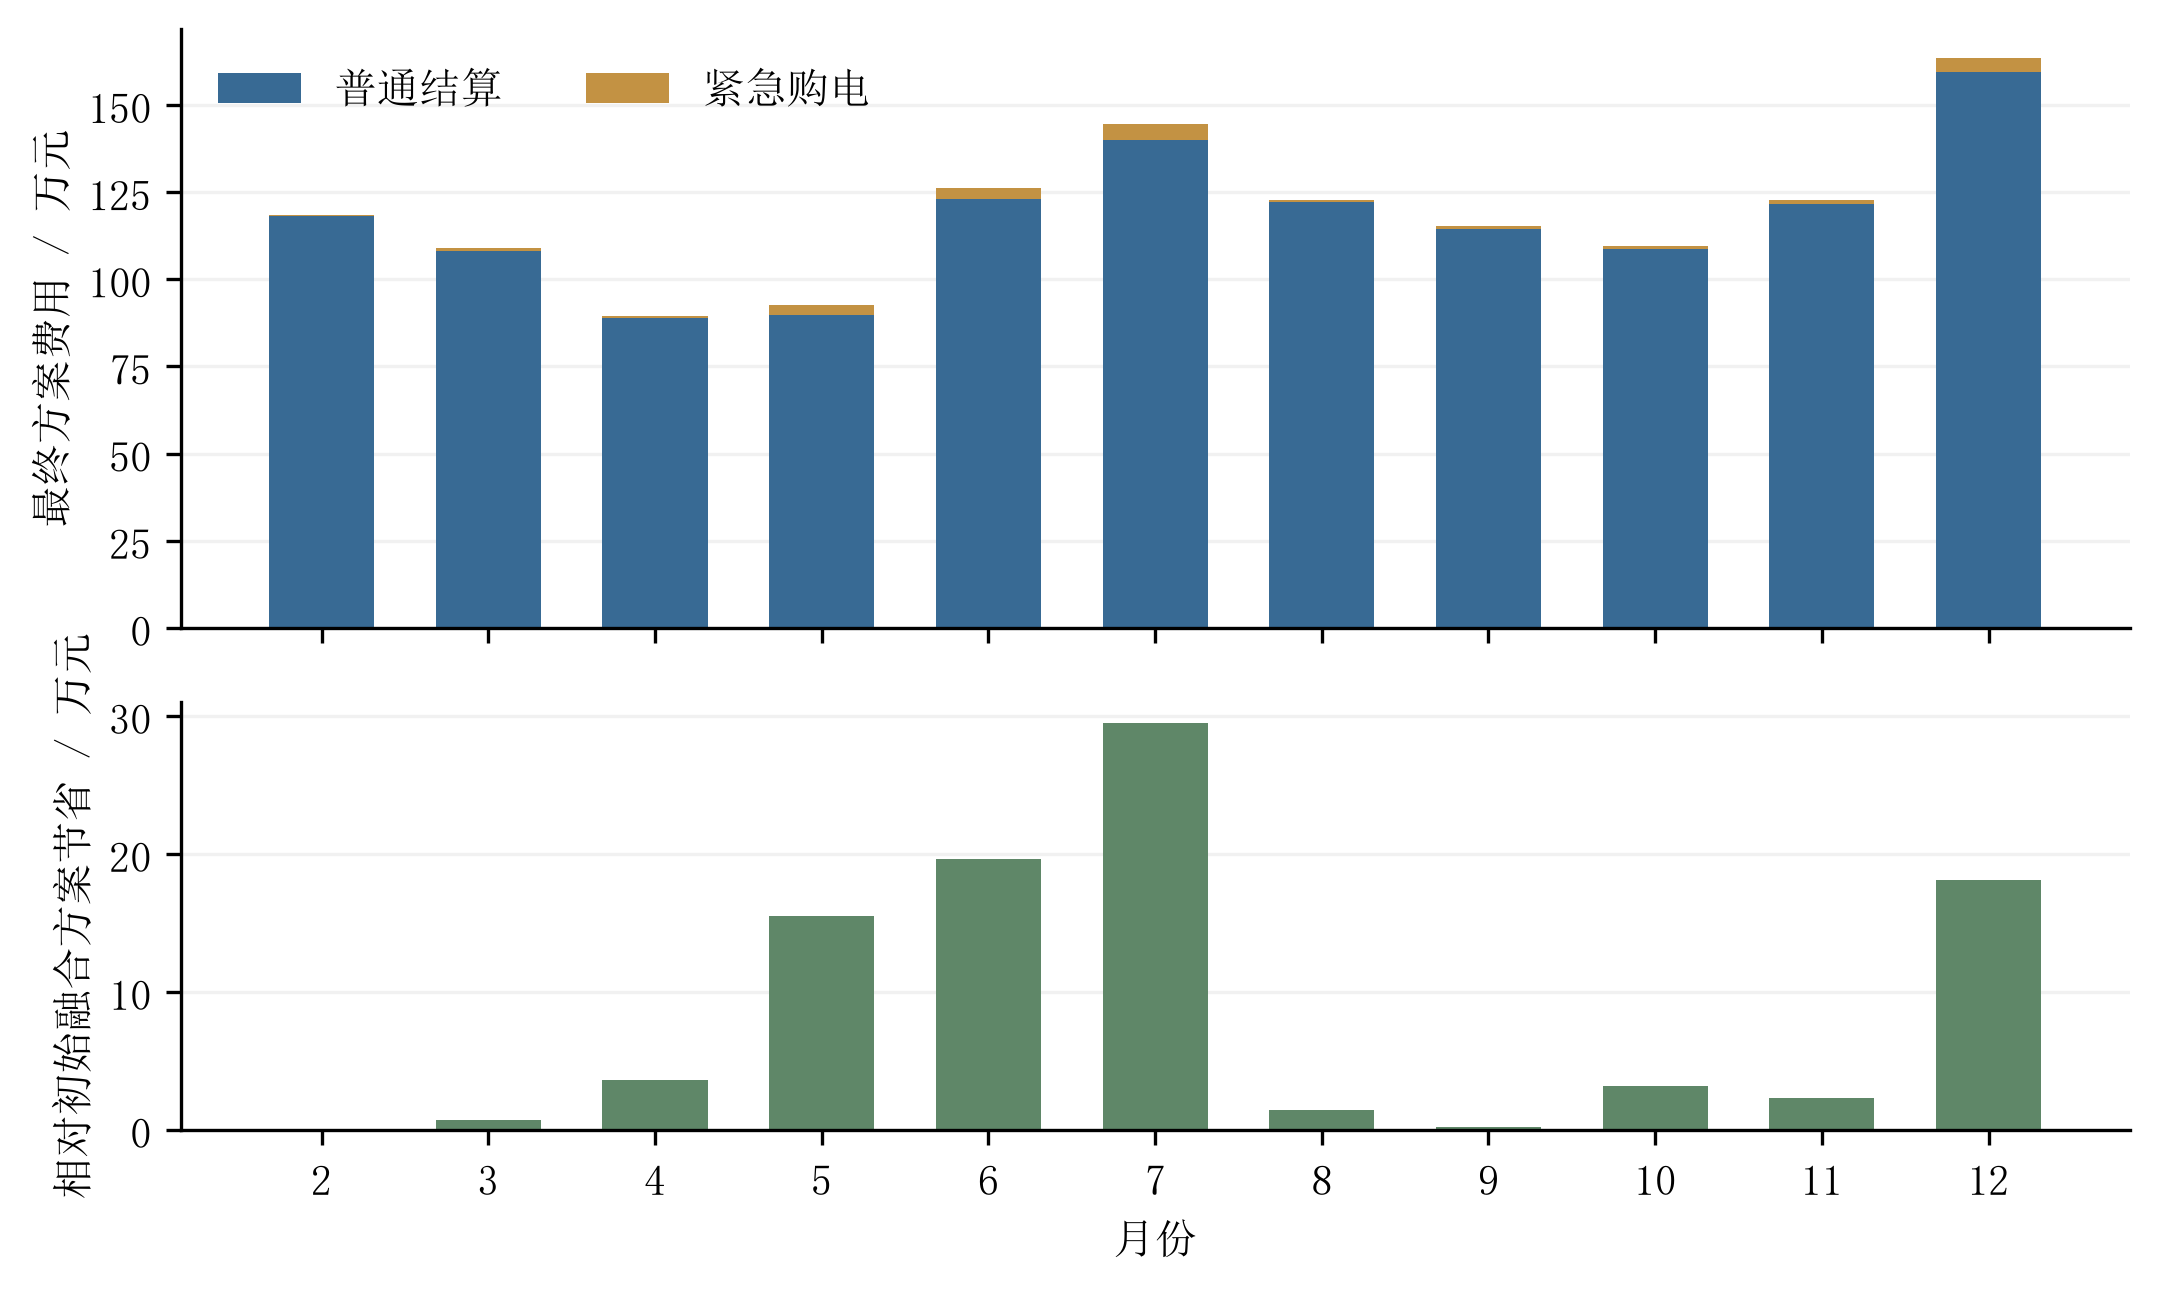
\includegraphics[width=0.90\textwidth]{fig/final_monthly.png}
    \caption{最终方案的月度费用及相对初始融合方案的节省}
    \label{fig:q3_monthly}
\end{figure}


\subsubsection*{（2）指定日期零点原计划}

题目指定日期在0:00制定的部分原始购电计划如表~\ref{tab:q3_original_order}所示。

\begin{table}[htbp]
\centering
\caption{指定日期零点原计划的部分时段购电量}
\label{tab:q3_original_order}
\begin{tabular}{ccccc}
\hline
时间段
& 3月20日
& 6月21日
& 9月23日
& 12月21日 \\
\hline
10:00--10:10 & 0.00   & 0.00   & 0.00   & 0.00 \\
12:00--12:10 & 586.14 & 0.00   & 436.19 & 948.82 \\
14:00--14:10 & 0.00   & 0.00   & 0.00   & 0.00 \\
16:00--16:10 & 489.39 & 110.71 & 472.88 & 806.52 \\
18:00--18:10 & 716.29 & 432.73 & 827.44 & 731.68 \\
20:00--20:10 & 0.00   & 0.00   & 5.90   & 0.00 \\
\hline
\end{tabular}
\end{table}


\subsubsection*{（3）日内调整后的购电结果}

经过6:00、12:00和18:00的滚动调整后，
指定日期的最终普通订单和全天费用如表~\ref{tab:q3_final_order}所示。

\begin{table}[htbp]
\centering
\caption{指定日期调整后订单及全天费用}
\label{tab:q3_final_order}
\begin{tabular}{lcccc}
\hline
项目
& 3月20日
& 6月21日
& 9月23日
& 12月21日 \\
\hline
10:00--10:10 & 0.00 & 0.00 & 0.00 & 0.00 \\
12:00--12:10 & 586.14 & 0.00 & 436.19 & 975.93 \\
14:00--14:10 & 0.00 & 0.00 & 0.00 & 0.00 \\
16:00--16:10 & 471.19 & 68.81 & 475.08 & 834.21 \\
18:00--18:10 & 716.29 & 424.29 & 809.29 & 731.64 \\
20:00--20:10 & 0.00 & 0.00 & 5.90 & 0.00 \\
\hline
全天原计划购电量/kWh
& 64012.35 & 39766.06 & 68933.65 & 94785.86 \\

全天最终普通订单/kWh
& 62868.01 & 39547.19 & 69071.70 & 95867.85 \\

全天紧急购电量/kWh
& 95.59 & 14.64 & 6.38 & 45.47 \\

普通结算费用/元
& 39587.60 & 21816.59 & 43609.00 & 62120.52 \\

紧急购电费用/元
& 666.80 & 58.34 & 43.00 & 198.32 \\

\textbf{全天总费用/元}
& \textbf{40254.40}
& \textbf{21874.93}
& \textbf{43652.00}
& \textbf{62318.84} \\
\hline
\end{tabular}
\end{table}

可以看出，日内调整并不是统一增加或减少购电量。
例如3月20日最终订单低于零点原计划，
而12月21日最终订单高于原计划，
说明模型会根据新的光伏信息和当前储电状态重新判断未来供需。


\subsubsection*{（4）指定日期储能运行}

四个指定日期的实际充放电及日首、日末储电量如表~\ref{tab:q3_storage}所示。

\begin{table}[htbp]
\centering
\caption{指定日期的实际充放电及日首尾储电量}
\label{tab:q3_storage}
\begin{tabular}{llcccc}
\hline
时间段 & 项目
& 3月20日
& 6月21日
& 9月23日
& 12月21日 \\
\hline
00:00--04:00 & 充电 & 1556.01 & 240.54  & 1739.21 & 2064.56 \\
              & 放电 & 185.93  & 348.67  & 2.78    & 215.12 \\

04:00--08:00 & 充电 & 951.71  & 257.49  & 57.67   & 1564.44 \\
              & 放电 & 5205.35 & 1744.95 & 6257.36 & 777.76 \\

08:00--12:00 & 充电 & 4142.68 & 10134.27 & 4754.81 & 4462.12 \\
              & 放电 & 3265.56 & 0.00     & 2387.94 & 8634.27 \\

12:00--16:00 & 充电 & 6169.03 & 344.79  & 6385.35 & 8760.52 \\
              & 放电 & 289.59  & 0.00    & 403.62  & 2070.34 \\

16:00--20:00 & 充电 & 138.06  & 83.56   & 94.38   & 7.92 \\
              & 放电 & 4894.55 & 5209.77 & 4784.01 & 5009.17 \\

20:00--24:00 & 充电 & 4405.05 & 8583.09 & 8446.30 & 8322.00 \\
              & 放电 & 3677.85 & 3028.38 & 3633.41 & 3628.73 \\
\hline
0:00  & 内部储电量 & 8873.79 & 3246.87 & 9214.11 & 8630.73 \\
24:00 & 内部储电量 & 5034.71 & 9446.49 & 9133.92 & 8699.27 \\
\hline
\end{tabular}
\end{table}

表中某个4小时区间同时存在充电量和放电量，
表示该区间内部不同的10分钟时段采取了不同动作，
并不表示储能设备在同一个10分钟时段同时充电和放电。


\subsubsection*{（5）紧急购电与典型日期分析}

指定日期的紧急购电结果如表~\ref{tab:q3_emergency}所示。

\begin{table}[H]
\centering
\caption{问题三指定日期的紧急购电量（kWh）}
\label{tab:q3_emergency}
\small
\setlength{\tabcolsep}{4pt}
\begin{tabular}{|c|c|c|c|c|c|c|c|}
\hline
\multicolumn{2}{|c|}{2025.3.20} & \multicolumn{2}{c|}{2025.6.21} & \multicolumn{2}{c|}{2025.9.23} & \multicolumn{2}{c|}{2025.12.21} \\
\hline
时间段 & 购电量 & 时间段 & 购电量 & 时间段 & 购电量 & 时间段 & 购电量 \\
\hline
20:40--20:50 & 95.59 & 07:20--07:30 & 14.64 & 20:30--20:40 & 6.38 & 08:00--08:10 & 9.20 \\
\hline
-- & -- & -- & -- & -- & -- & 10:50--11:00 & 36.26 \\
\hline
\end{tabular}
\end{table}
表中各时段电量分别保留两位小数，全天合计由未舍入的逐段结果计算，因此显示值相加可能与全天合计存在0.01 kWh的差异。

图~\ref{fig:q3_days}进一步展示了3月20日和9月23日的实际负载、
实际光伏、零点订单、最终订单、储电状态以及缺口补充过程。

3月20日20:40附近，电池已经接近1200~kWh的储电下限，
仍有95.59~kWh缺口无法继续由储能补足，因此需要紧急购电。
9月23日仅在20:30--20:40发生6.38~kWh紧急购电。

这说明是否需要紧急购电不能只比较全天总电量，
还必须考虑缺口出现的具体时刻、当时剩余储电量以及储能设备的放电能力。

\begin{figure}[H]
    \centering
    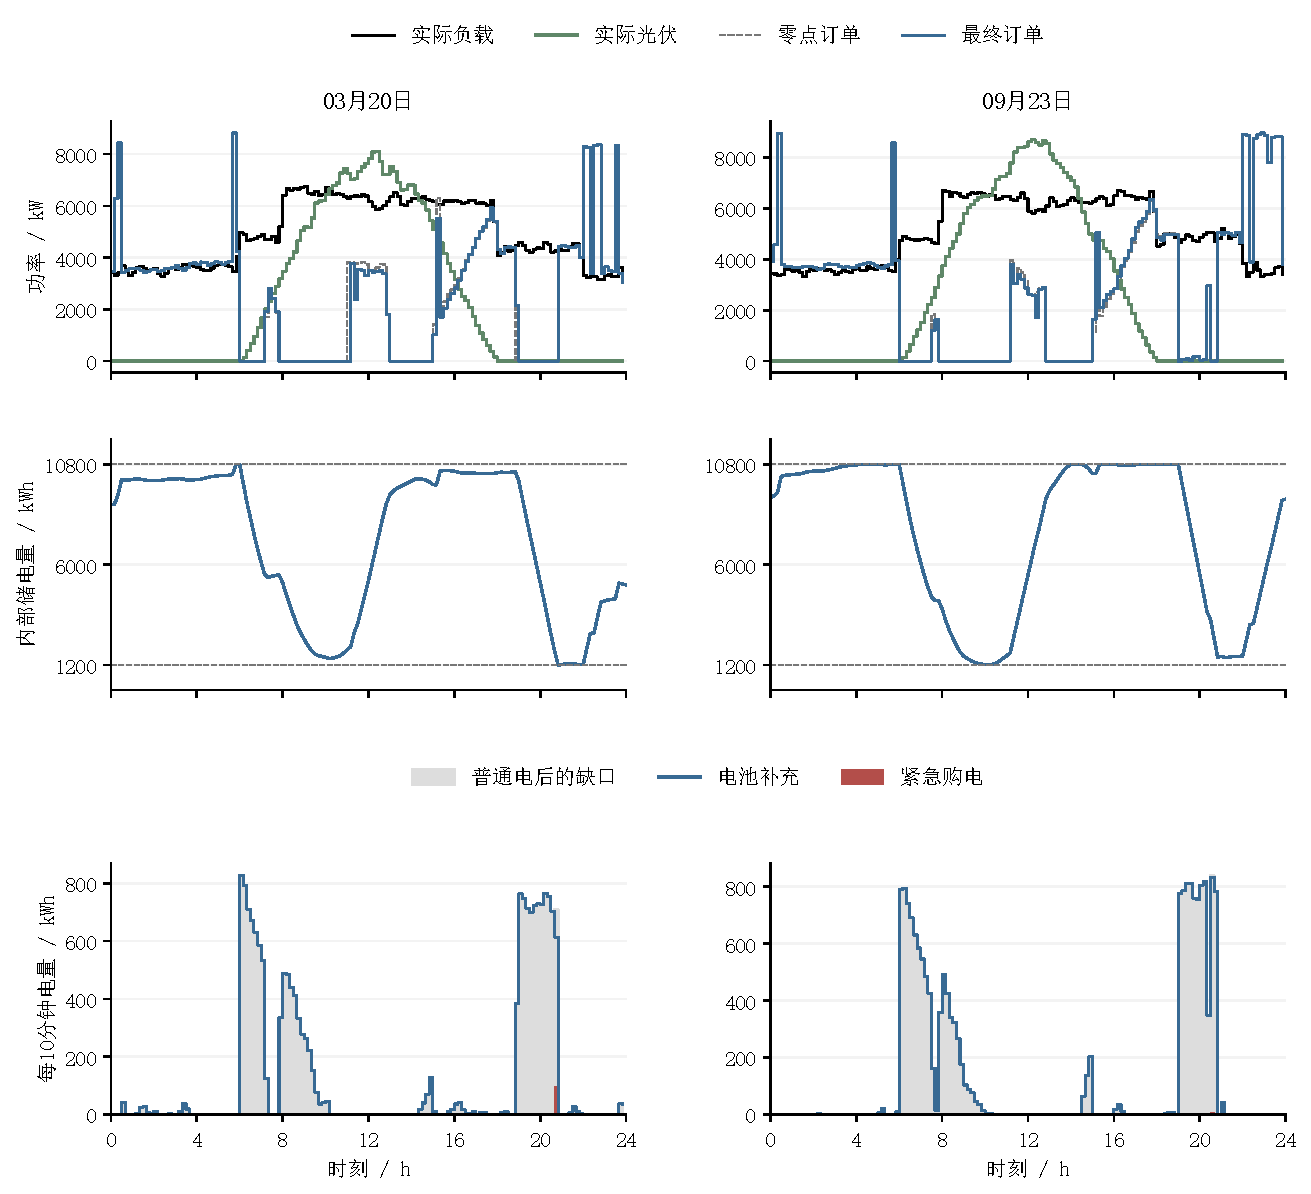
\includegraphics[width=0.95\textwidth]{fig/q3_specified_days.pdf}
    \caption{两个指定日期的供需、库存和缺口补充过程}
    \label{fig:q3_days}
\end{figure}


\subsection{日内新预报的实际费用价值}

题目要求判断是否有必要使用6:00、12:00和18:00的新光伏预报。

若直接比较零点固定订单与完整问题三方案，
会同时混入日内实际供需反馈、真实储电量更新和新官方预报三种作用。
因此，在直接使用官方预报的同一策略下设置三个逐步增加信息的对照方案，
结果如表~\ref{tab:q3_info}和图~\ref{fig:q3_info}所示。

\begin{table}[H]
\centering
\caption{日内反馈与新增官方预报的费用比较}
\label{tab:q3_info}
\begin{tabular}{lc}
\hline
方案 & 总费用/万元 \\
\hline
零点订电，全天不修改订单
& 1614.80 \\

允许日内反馈和改单，但不使用后发官方预报
& 1439.29 \\

允许日内反馈和改单，并使用新官方预报
& 1417.51 \\
\hline
\end{tabular}
\end{table}

开放日内实际反馈和订单调整后，
总费用首先减少175.51万元；
在相同的反馈和改单权限下，
进一步使用6:00、12:00和18:00的新官方预报，
又减少21.78万元。

因此，对于题目提出的“是否需要引入其他时刻预报”，本文认为
\[
\boxed{\text{需要引入日内新预报}}.
\]

在相同反馈和调整条件下，
使用新官方预报将费用由1439.29万元降低至1417.51万元，
额外节省21.78万元，约为1.51\%。

但这并不表示三个发布时间具有完全相同的价值，
也不表示每次收到新预报后都必须修改订单。
是否改单仍需结合预测变化、调整费用和当前储电状态共同决定。

\begin{figure}[H]
    \centering
    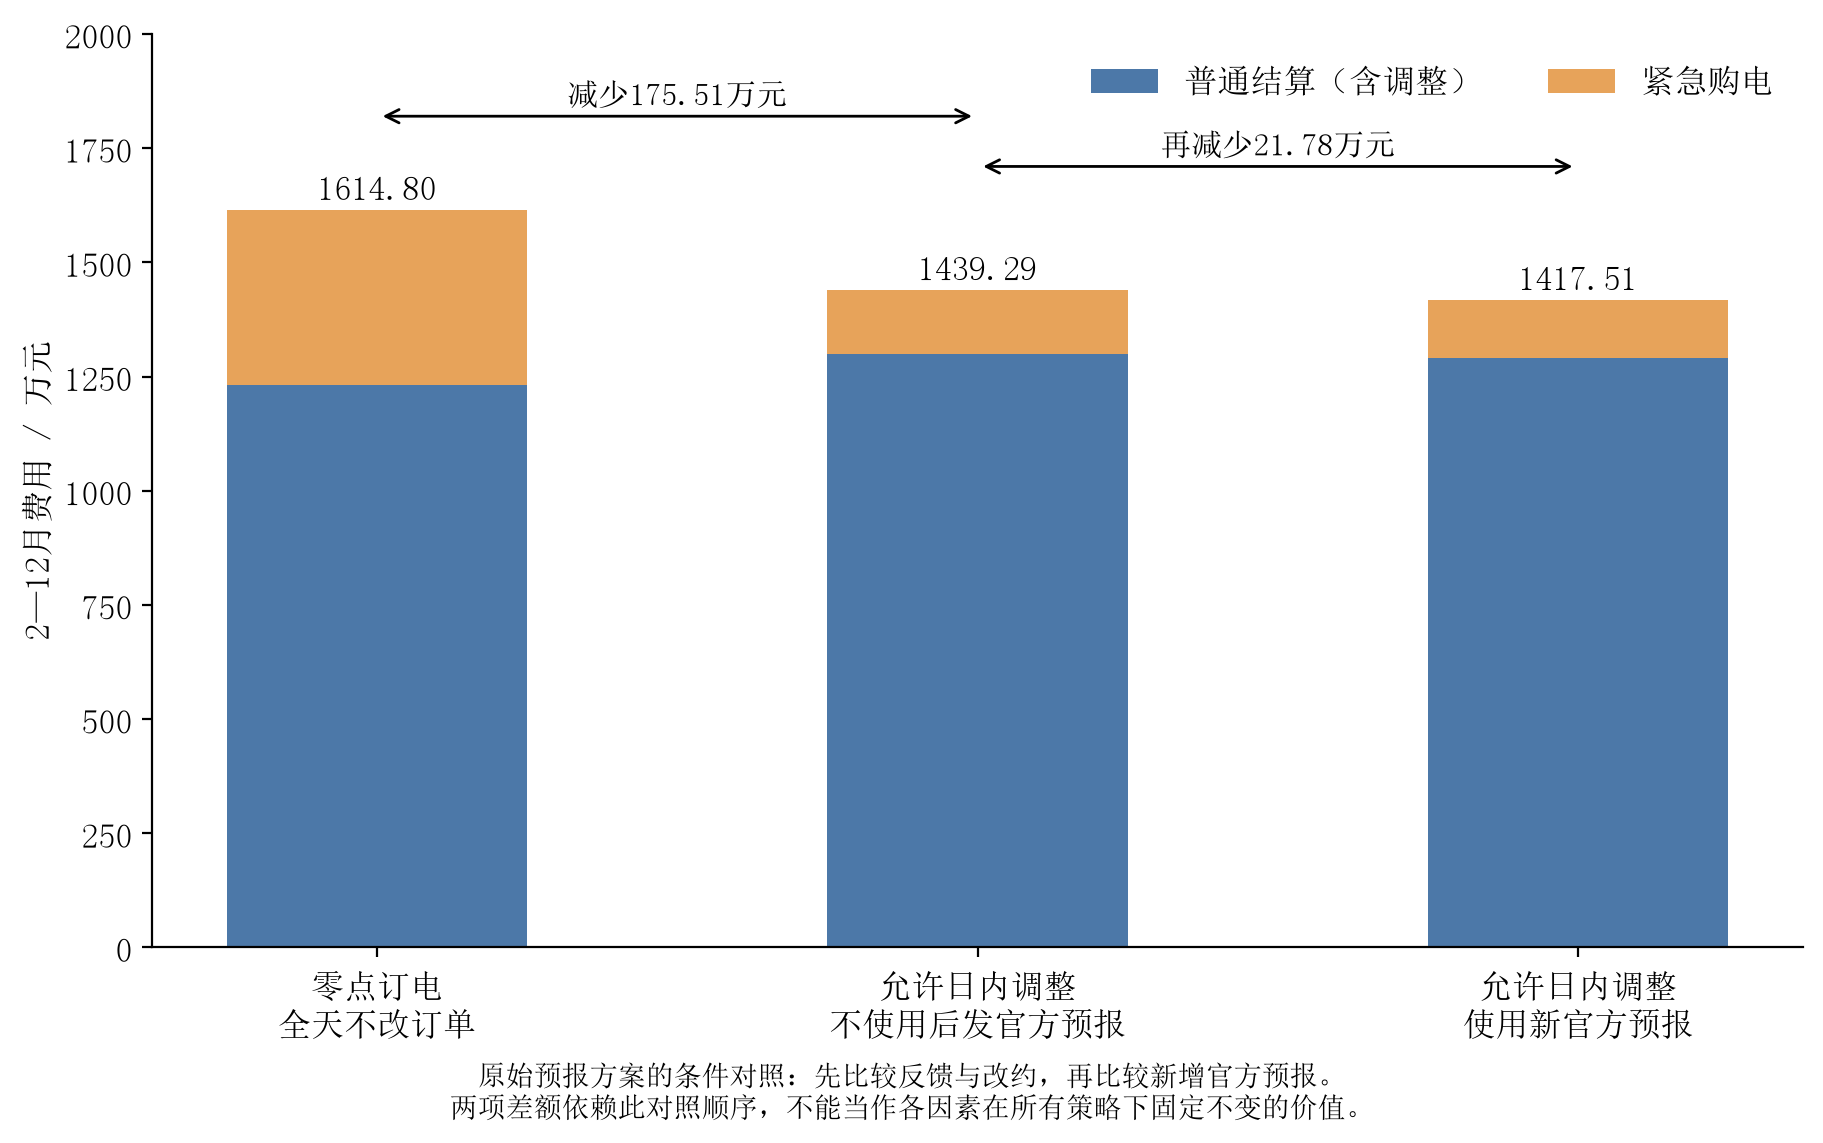
\includegraphics[width=0.85\textwidth]{fig/information_value.png}
    \caption{日内反馈、改单与新增官方预报的费用价值}
    \label{fig:q3_info}
\end{figure}


\subsection{参数灵敏度与模型可信度}

动态安全准备量依赖误差分位、日期衰减、误差分组宽度和历史窗口。
为了避免参数选择过于主观，
本文在其他条件保持不变的情况下分别进行灵敏度比较，
结果如图~\ref{fig:q3_parameter}所示。

\subsubsection*{（1）误差分位}

在0.55--0.80的分位范围内，
0.60对应的全年总费用最低。
继续提高分位虽然能够减少紧急购电，
但普通购电和未接收订单随之增加，
最终总费用反而上升。

\subsubsection*{（2）日期衰减}

时间衰减参数分别取0.7、0.8和1.0时，
总费用约为
\[
1314.65,\qquad
1318.88,\qquad
1342.54
\quad \text{万元}.
\]

因此，近期误差应在当前购电决策中发挥更大的作用，
最终取衰减参数为0.7。

\subsubsection*{（3）误差分组宽度}

比较1、2、3、4和6小时的误差分组后，
3小时方案总费用最低。
同时，3小时恰好将每个6小时预报更新区间划分为前后两段，
能够兼顾日内误差差异与历史样本稳定性。

\subsubsection*{（4）历史窗口}

历史窗口分别取14、28和56天时，
相对于28天方案的费用差仅为十余元。
因此，模型对这一参数并不敏感，
最终采用能够覆盖4个完整星期的28天历史窗口。

此外，逐次撤去安全准备量以及强制保留零点订单一定比例的方案均会增加总费用。
因此，最终模型在0:00、6:00、12:00和18:00四次决策中均重新计算并保留安全准备，
同时不额外限制向下调整订单的比例，
而由模型根据新预报、调整费用和真实库存自行决定是否改单。

\begin{figure}[H]
    \centering
    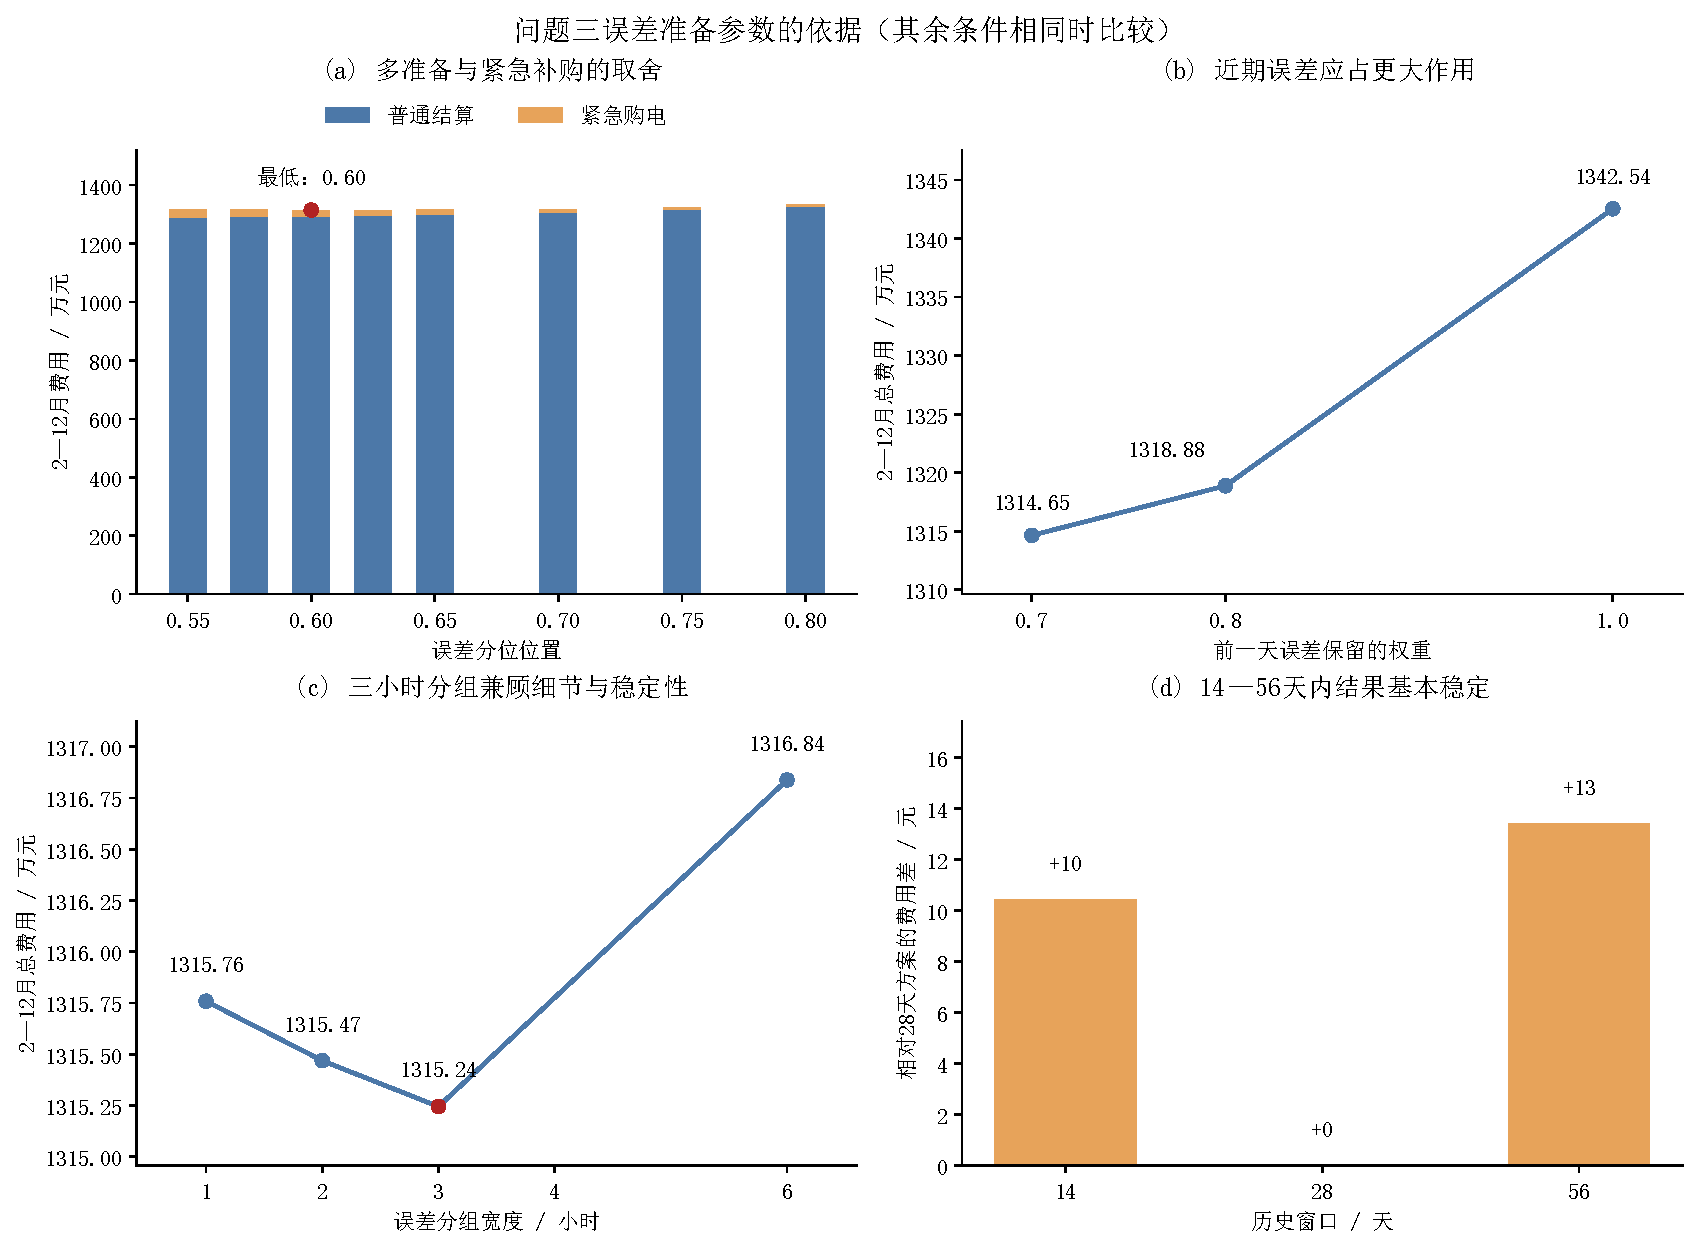
\includegraphics[width=0.95\textwidth]{fig/q3_parameter_interpretability.pdf}
    \caption{近期误差准备参数的费用依据}
    \label{fig:q3_parameter}
\end{figure}

为检验计算结果，对保存的策略重新计算逐10分钟供需、
储电状态、充放电功率、订单锁定和总费用。
费用最大复算误差约为
\[
1.9\times10^{-9}\ \text{元},
\]
各项储能和供电约束均得到满足。

需要说明的是，上述参数是在题目给出的2025年数据范围内比较得到，
能够支持本年度条件下的模型选择与费用分析；
若用于其他年份或其他微网，仍需结合新的运行数据重新校准。
